% !TEX root = main.tex
\documentclass{article}

% =========================================================
% NeurIPS 2026 style
% =========================================================

% Submission (anonymous, with line numbers):
\usepackage{neurips_2026}

% Camera-ready:
% \usepackage[main, final]{neurips_2026}

% Preprint / arXiv:
% \usepackage[preprint]{neurips_2026}

% If natbib conflicts:
% \usepackage[nonatbib]{neurips_2026}

% =========================================================
% Basic packages from template
% =========================================================
\usepackage{iftex}
\ifPDFTeX
  \usepackage[utf8]{inputenc}
\fi
\usepackage[T1]{fontenc}
\usepackage{hyperref}
\usepackage{url}
\usepackage{booktabs}
\usepackage{amsfonts}
\usepackage{nicefrac}
\usepackage{microtype}
\usepackage{xcolor}

% =========================================================
% Recommended math / figure / table packages
% =========================================================
\usepackage{amsmath, amssymb, amsthm, mathtools}
\usepackage{graphicx}
\usepackage{caption}
\usepackage{subcaption}
\usepackage{multirow}
\usepackage{array}
\usepackage{siunitx}
\usepackage{enumitem}
\usepackage{wrapfig}

% Optional but useful
\usepackage[nameinlink,capitalize,noabbrev]{cleveref}

% =========================================================
% Macros
% =========================================================
% =========================================================
% Math shortcuts
% =========================================================
\newcommand{\R}{\mathbb{R}}
\newcommand{\E}{\mathbb{E}}
\newcommand{\Prob}{\mathbb{P}}

\newcommand{\bx}{\mathbf{x}}
\newcommand{\bw}{\mathbf{w}}
\newcommand{\btheta}{\boldsymbol{\theta}}

\newcommand{\method}{\textsc{YourMethod}}
\newcommand{\dataset}{\textsc{YourDataset}}

% =========================================================
% Ref helpers
% =========================================================
\newcommand{\figref}[1]{Fig.~\ref{#1}}
\newcommand{\tabref}[1]{Table~\ref{#1}}
\newcommand{\secref}[1]{Sec.~\ref{#1}}
\newcommand{\appref}[1]{App.~\ref{#1}}

% =========================================================
% Comments (turn off before submission if needed)
% =========================================================
\newcommand{\todo}[1]{\textcolor{red}{[TODO: #1]}}
\newcommand{\scholarcite}[2]{\href{https://scholar.google.com/scholar?q=#1}{\citep{#2}}}

% =========================================================
% Metadata
% =========================================================
\title{Disentangled Knowledge in Diffusion Transformer}

\author{%
  Anonymous Authors \\
  Anonymous Institution \\
  Anonymous Email
}

\begin{document}

\maketitle

\begin{abstract}
Intermediate representations are increasingly recognized as a key factor in the training dynamics and generation quality of Diffusion Transformers (DiTs). Existing self-guided methods such as layer synchronization and self-representation alignment improve these representations by directly aligning selected internal features, but they provide limited supervision on how hidden states evolve across depth. We propose \emph{ReSync}, a self-supervised objective for self-aligned representation transition consistency in DiTs. Given a source hidden state, source and target layer indices, and the diffusion timestep, a lightweight transition predictor estimates the target-layer representation. The predictor is trained with grounded layer alignment and bootstrap transition consistency, encouraging composed short transitions to match direct long transitions. Rather than treating cross-layer similarity as the objective itself, ReSync learns a conditional hidden-state transport model, providing dense supervision over the DiT depth trajectory while preserving layer-specific transformations. We further introduce an optional output distillation loss that makes predicted skipped states useful for the final velocity prediction, enabling a natural quality--speed tradeoff through layer skipping. Experiments show that ReSync improves representation learning and generative performance.

\end{abstract}

\begin{figure}[!htbp]
  \centering
  \begin{subfigure}[t]{0.39\textwidth}
    \centering
    \fbox{%
      \begin{minipage}[c][0.23\textheight][c]{0.92\linewidth}
        \centering
        \textbf{Architecture placeholder}\\[0.5em]
        Insert DSP overview here:\\
        DiT hidden-state trajectory,\\
        depth shortcut predictor,\\
        direct supervision, and\\
        bootstrap depth consistency.
      \end{minipage}%
    }
    \caption{Model architecture.}
    \label{fig:overview_architecture}
  \end{subfigure}
  \hfill
  \begin{subfigure}[t]{0.56\textwidth}
    \centering
    \fbox{%
      \begin{minipage}[c][0.23\textheight][c]{0.94\linewidth}
        \centering
        \textbf{Training graph placeholder}\\[0.5em]
        Insert convergence plot here:\\
        baseline vs. DSP training curves,\\
        e.g., FID or validation loss\\
        over training iterations.
      \end{minipage}%
    }
    \caption{Training dynamics.}
    \label{fig:overview_training}
  \end{subfigure}
  \caption{\textbf{Depth Shortcut Prediction improves diffusion-transformer training through internal cross-depth supervision.}
  (a) DSP learns conditional transitions between intermediate DiT hidden states using a lightweight shortcut predictor, with direct cross-layer targets and bootstrap consistency across composed depth transitions.
  (b) The same auxiliary signal is expected to improve training dynamics, shown as a placeholder for convergence curves comparing the baseline backbone and the DSP-augmented model.}
  \label{fig:dsp_overview}
\end{figure}

\clearpage

\section{Introduction}

Denoising-based generative models, including diffusion models~\citep{ho2020ddpm,song2021score,song2020sde} and flow matching models~\citep{lipman2022flow}, have achieved remarkable success in high-fidelity image generation. Among them, Diffusion Transformers (DiTs) have become a particularly scalable backbone due to their strong modeling capacity and compatibility with large-scale training. Despite these advances, training DiTs remains computationally expensive, and improving their optimization efficiency without sacrificing generation quality is still an important challenge.

A growing body of work suggests that the intermediate representations of diffusion transformers play a critical role in both training dynamics and final generation quality. Representation alignment methods such as REPA~\citep{yu2024repa} show that aligning DiT hidden states with strong visual representations from pretrained encoders can substantially accelerate training. Subsequent studies further indicate that the benefit of such alignment is closely tied to the structure and quality of intermediate features, motivating a broader view that improving internal representations can be an effective route to improving generative modeling. However, these methods often rely on external representation encoders, which introduce additional computation, architectural dependency, and reduced portability to domains where strong pretrained teachers are unavailable.

Recent self-contained methods attempt to remove this dependency by using the diffusion transformer itself as a source of representation guidance. SRA~\citep{jiang2025sra} observes that representations in diffusion transformers tend to improve as noise decreases and depth increases, and therefore aligns earlier or noisier features with later or cleaner features from an EMA teacher. LayerSync~\citep{haghighi2026layersync} similarly exploits cross-layer structure by encouraging shallow representations to synchronize with deeper, more informative ones. These works suggest that useful supervision already exists inside the model: different layers and timesteps provide different views of the same denoising process, and this internal structure can guide representation learning without an external teacher.

Nevertheless, directly aligning hidden states is only one way to exploit cross-layer information. Inspired by shortcut models and consistency-style learning, we ask whether the evolution of DiT representations across depth can itself be used as a training signal. Rather than simply forcing two layers to be close, we learn a conditional transition between them: given a hidden state at an earlier layer, a lightweight predictor estimates the corresponding representation at a later layer. This turns the DiT depth trajectory into a self-supervised representation learning problem. A useful intermediate representation should not only support the final denoising or velocity prediction, but should also evolve in a predictable and compositional manner across transformer depth.

To this end, we propose \emph{Depth Shortcut Prediction} (DSP), a self-contained auxiliary objective for diffusion transformers. DSP trains a lightweight predictor to map a source-layer hidden state to a target-layer hidden state conditioned on the source layer, target layer, and timestep. To handle the scale variation of hidden states, we formulate prediction in direction--magnitude space: the predictor estimates both the target token directions and the residual change in log magnitude. The training objective consists of two auxiliary losses, one for direction prediction and one for magnitude prediction. Each loss combines direct cross-depth supervision with a bootstrap consistency term, encouraging composed short transitions to agree with direct long transitions.

Our method is designed primarily as a representation learning objective. By supervising cross-depth prediction over many layer pairs, DSP encourages the DiT backbone to learn intermediate features whose evolution is structured, predictable, and useful for generation. As a secondary consequence, the learned predictor can also reconstruct skipped hidden states and enable optional layer-skipping inference, providing a controllable quality--speed tradeoff. However, unlike methods focused purely on efficient inference, our main goal is to improve representation quality and generative training using the model's own hidden-state trajectory.

Our main contributions are as follows:
\begin{itemize}
    \item We introduce Depth Shortcut Prediction, a self-supervised representation learning objective that uses cross-depth hidden-state prediction as internal guidance for diffusion transformers.

    \item We formulate hidden-state prediction in direction--magnitude space, allowing the model to learn both target representation orientation and scale through two auxiliary losses.

    \item We incorporate bootstrap depth consistency, encouraging learned transitions to be compositional across transformer depth rather than only fitting isolated layer pairs.

    \item We show that the resulting objective improves DiT representation learning and generation quality, while also enabling optional layer-skipping inference as an auxiliary benefit.
\end{itemize}
\section{Related Work}

\noindent\textbf{Representation guidance for diffusion transformers.} Recent work shows that diffusion and flow-based generative models learn intermediate representations whose quality is closely tied to generative performance~\citep{mukhopadhyay2024, kim2025, stracke2025, yu2024repa}. REPA improves DiT and SiT training by aligning hidden states with external visual representations from pretrained encoders~\citep{yu2024repa}, and follow-up methods further refine this alignment paradigm through stronger training recipes or more spatially faithful targets~\citep{wang2025haste,leng2025repae,singh2025irepa}. These methods are effective, but their dependence on external teachers introduces additional computation, architectural coupling, and limited portability to domains where strong pretrained encoders are unavailable~\citep{oquab2023dinov2,yu2024repa}.

\noindent\textbf{Self-contained internal alignment.} To remove external encoders, SRA aligns earlier or noisier features with later or cleaner features from an EMA teacher built from the diffusion model itself~\citep{jiang2025sra}. LayerSync similarly uses deeper, more informative internal layers as intrinsic guidance for weaker shallow layers~\citep{haghighi2026layersync}. Complementary work also suggests that excessive layer similarity can hurt specialization, motivating regularizers that preserve diversity across blocks~\citep{wang2025dispersive,yang2026diversedit}. ReSync follows the self-contained direction of SRA and LayerSync, but replaces direct pairwise alignment with a learned transition model over depth. Rather than only encouraging two layers to be similar, ReSync learns how representations should move from $h_a$ to $h_b$ and enforces that these transitions compose consistently across layers.

\section{Method}
\label{sec:method}

\subsection{Preliminaries}

We describe ReSync on top of a diffusion-transformer backbone trained with a standard diffusion or flow-matching objective. For concreteness, we use the stochastic-interpolant formulation of SiT~\citep{ma2024sit}. Given data $x_0$, noise $\epsilon$, and timestep $t$, the model observes
\begin{equation}
x_t=\alpha_t x_0+\sigma_t\epsilon .
\label{eq:stochastic_interpolant}
\end{equation}
Let $u_t=\dot{\alpha}_t x_0+\dot{\sigma}_t\epsilon$ be the corresponding velocity target. The backbone $f_\zeta$ and output head $v_\zeta$ are trained with
\begin{equation}
\mathcal{L}_{\mathrm{gen}}
=
\mathbb{E}_{x_0,\epsilon,t}
\left[
\left\|v_\zeta(x_t,t,c)-u_t\right\|_2^2
\right].
\label{eq:flow_matching_loss}
\end{equation}
During the same forward pass, the transformer exposes hidden states $h_0(t),\ldots,h_L(t)$, where $h_\ell(t)$ denotes the representation after block $\ell$. ReSync adds training-time losses on these states. The sampling network is unchanged unless the optional layer-skipping branch is enabled.

\subsection{ReSync: Learning Internal Transitions}

Representation alignment methods usually choose a source representation and a target representation, optionally insert a projection head, and then minimize a similarity loss. REPA uses external targets, while SRA and LayerSync show that useful targets can also come from the diffusion model itself~\citep{yu2024repa,jiang2025sra,haghighi2026layersync}. Projection heads can be viewed as practical adapters for matching different representation spaces, but when an adapter is tied to a fixed pair it remains a local solution.

ReSync turns this local adapter into a shared transition model. For two layers $a<b$, we predict the later hidden state from the earlier one as
\begin{equation}
\hat h_b(t)=T_\psi(h_a(t);a,b,t),
\label{eq:resync_predictor}
\end{equation}
where $T_\psi$ is a lightweight predictor conditioned on the source layer, target layer, and timestep. The same predictor is reused across sampled layer pairs, so the auxiliary task is not simply to fit one projection head for one target. Instead, it asks the model to learn reusable changes between internal representation spaces. A cross-timestep variant can replace the target $h_b(t)$ with a cleaner or noisier state from the same sample, following the spirit of SRA; we keep the same-timestep form as the main objective for clarity and lower training cost.

\subsection{Grounded and Compositional Objectives}

The grounded transition loss uses the real target hidden state as a detached supervision signal:
\begin{equation}
\mathcal{L}_{\mathrm{align}}
=
\mathbb{E}_{a<b,t}
\left[
d\left(T_\psi(h_a(t);a,b,t),\mathrm{sg}(h_b(t))\right)
\right],
\label{eq:align_loss}
\end{equation}
where $\mathrm{sg}(\cdot)$ denotes stop-gradient and $d$ is a tokenwise distance, cosine distance by default. This term provides the same kind of internal guidance as self-alignment, but the source layer is not forced to match the target layer in raw feature coordinates.

Grounded prediction alone could still be solved by pair-specific shortcuts. ReSync therefore requires transitions to compose across depth. For layers $a<b<c$, the transition obtained by going through $b$ should agree with the direct transition from $a$ to $c$. We implement this with an EMA copy $\overline{T}_\psi$ as the bootstrap target:
\begin{equation}
\mathcal{L}_{\mathrm{cons}}
=
\mathbb{E}_{a<b<c,t}
\left[
d\left(
T_\psi(T_\psi(h_a(t);a,b,t);b,c,t),
\mathrm{sg}\left(\overline{T}_\psi(h_a(t);a,c,t)\right)
\right)
\right].
\label{eq:consistency_loss}
\end{equation}
This consistency term is the key distinction from a collection of projection heads. It couples short and long transitions, encouraging a shared internal dynamics rather than independent alignment rules for isolated layer pairs.

\subsection{Optional Output Distillation and Training Objective}

ReSync can also be used to test layer-skipping behavior. Given a predicted state $\hat h_b(t)$, we resume the remaining blocks and output head $F_{b+1:L}$:
\begin{equation}
\hat y_{\mathrm{skip}}
=
F_{b+1:L}(\hat h_b(t),t,c).
\label{eq:skip_output}
\end{equation}
The skipped output is matched to the full model output,
\begin{equation}
\mathcal{L}_{\mathrm{out}}
=
\left\|
\hat y_{\mathrm{skip}}
-
\mathrm{sg}(\hat y_{\mathrm{full}})
\right\|_2^2 .
\label{eq:output_distillation_loss}
\end{equation}
We treat this term as optional; the main claim of ReSync is representation regularization through transition prediction and compositional consistency.

The final objective is
\begin{equation}
\mathcal{L}
=
\mathcal{L}_{\mathrm{gen}}
+
\lambda_{\mathrm{align}}\mathcal{L}_{\mathrm{align}}
+
\lambda_{\mathrm{cons}}\mathcal{L}_{\mathrm{cons}}
+
\lambda_{\mathrm{out}}\mathcal{L}_{\mathrm{out}} .
\label{eq:total_loss}
\end{equation}
When $\lambda_{\mathrm{out}}=0$, ReSync is purely a training-time self-distillation objective and adds no inference-time computation.

\section{Experiments}
\label{sec:experiments}

This section evaluates whether \emph{ReSync} improves diffusion-transformer training by using the model's own cross-depth representation dynamics as self-aligned transition supervision. Our experiments are organized around four questions:
\begin{itemize}[leftmargin=*]
    \item Which components of ReSync are most important for generation quality and training efficiency? See \Cref{tab:resync_ablation}.
    \item Does ReSync remain effective across different backbone families and model scales? See \Cref{fig:training_curves,tab:model_scaling}.
    \item How does ReSync compare with methods that rely on external representation tasks or pretrained representation encoders? See \Cref{tab:comparison_external_guidance}.
    \item Does ReSync actually improve the representation capacity of the backbone, and how strongly is this improvement correlated with generation quality? See \Cref{fig:representation_analysis}.
\end{itemize}

\subsection{Experimental Setup}
\label{sec:experimental_setup}

\paragraph{Implementation details.}
Unless otherwise stated, we follow the standard latent diffusion-transformer training recipe used by DiT and SiT-style baselines~\citep{ma2024sit}. Models are trained with AdamW using a constant learning rate of $10^{-4}$, no weight decay, and a batch size of $256$. Images are encoded into latent space using the Stable Diffusion VAE, and we evaluate the \texttt{B/2}, \texttt{L/2}, and \texttt{XL/2} model configurations with patch size $2$. For ReSync, the transition predictor is trained jointly with the backbone using the auxiliary objective in \Cref{eq:total_loss}. We leave dataset-specific details, training length, transition-pair sampling, EMA decay, loss weights, and compute budget as explicit placeholders: \textbf{[PLACEHOLDER: dataset, resolution, number of iterations, hardware, $\lambda_{\mathrm{align}}$, $\lambda_{\mathrm{cons}}$, $\lambda_{\mathrm{out}}$, EMA decay, and predictor architecture details]}.

\paragraph{Evaluation.}
We report standard image-generation metrics, including Frechet Inception Distance (FID), sFID, Inception Score (IS), precision, and recall. Unless otherwise specified, metrics are computed using $50\mathrm{K}$ generated samples and the same reference statistics as prior diffusion-transformer work. We will use a consistent evaluation implementation for all baselines and ReSync variants. \textbf{[PLACEHOLDER: cite and specify the exact evaluation suite, e.g., ADM TensorFlow evaluator or another agreed protocol.]}

\paragraph{Comparison methods.}
We compare ReSync against representative generative baselines from three groups: pixel-space diffusion models, latent diffusion models with convolutional U-Net backbones, and latent diffusion models with transformer backbones. The main comparison set should include the base DiT/SiT backbone, recent acceleration or representation-guidance methods such as REPA, SRA, LayerSync, and other transformer-based diffusion baselines when available. To keep the comparison focused, we separate methods that primarily introduce new architecture designs from methods that modify the training objective or representation guidance. \textbf{[PLACEHOLDER: finalize baseline list and add citations for ADM, LDM, DiT, SiT, REPA, SRA, LayerSync, MaskDiT, TREAD, MAETok, and any architecture-focused models to exclude or discuss separately.]}

\subsection{Ablation Study}
\label{sec:ablation_study}

We first isolate the contribution of each ReSync design choice. The ablation should start from the same backbone trained without the ReSync objective, then add direct cross-depth transition prediction, bootstrap transition consistency, EMA bootstrap targets, and optional output distillation. This study tests whether the benefit comes from a single alignment loss or from modeling cross-layer transitions as a compositional prediction problem.

\begin{table}[t]
    \centering
    \caption{\textbf{Ablation of ReSync components.} Placeholder table for measuring how each component affects generation quality and training efficiency. Lower FID/sFID is better; higher IS, precision, and recall are better.}
    \label{tab:resync_ablation}
    \resizebox{\textwidth}{!}{%
    \begin{tabular}{lcccccc}
        \toprule
        Method variant & Align & Consistency & EMA target & Output distill. & FID $\downarrow$ & IS $\uparrow$ \\
        \midrule
        Baseline backbone & -- & -- & -- & -- & \textbf{[TBD]} & \textbf{[TBD]} \\
        + transition alignment & \checkmark & -- & -- & -- & \textbf{[TBD]} & \textbf{[TBD]} \\
        + transition consistency & \checkmark & \checkmark & -- & -- & \textbf{[TBD]} & \textbf{[TBD]} \\
        + EMA target & \checkmark & \checkmark & \checkmark & -- & \textbf{[TBD]} & \textbf{[TBD]} \\
        Full ReSync & \checkmark & \checkmark & \checkmark & \checkmark & \textbf{[TBD]} & \textbf{[TBD]} \\
        \bottomrule
    \end{tabular}}
\end{table}

\subsection{Scaling Across Backbones and Model Sizes}
\label{sec:scaling_experiments}

Next, we evaluate whether ReSync is robust to changes in model capacity and baseline choice. The expected comparison includes at least \texttt{B/2}, \texttt{L/2}, and \texttt{XL/2} variants, each trained with and without ReSync under the same recipe. The key question is whether cross-depth transition supervision provides a consistent gain rather than only improving one specific configuration.

\begin{figure}[t]
    \centering
    \fbox{%
    \begin{minipage}[c][0.23\textheight][c]{0.88\linewidth}
        \centering
        \textbf{[PLACEHOLDER: training curves]}\\[0.5em]
        Plot baseline vs. ReSync across training iterations.\\
        Suggested axes: training iterations on the $x$-axis and FID, validation loss, or representation metric on the $y$-axis.
    \end{minipage}}
    \caption{\textbf{Training dynamics across model scales.} Placeholder for convergence curves comparing baseline backbones and ReSync-augmented backbones.}
    \label{fig:training_curves}
\end{figure}

\begin{table}[t]
    \centering
    \caption{\textbf{ReSync across model sizes.} Placeholder table for comparing baseline and ReSync variants under matched training settings.}
    \label{tab:model_scaling}
    \begin{tabular}{lcccc}
        \toprule
        Backbone & Params & Objective & FID $\downarrow$ & Throughput / steps \\
        \midrule
        \texttt{B/2} & \textbf{[TBD]} & Baseline & \textbf{[TBD]} & \textbf{[TBD]} \\
        \texttt{B/2} & \textbf{[TBD]} & Baseline + ReSync & \textbf{[TBD]} & \textbf{[TBD]} \\
        \texttt{L/2} & \textbf{[TBD]} & Baseline & \textbf{[TBD]} & \textbf{[TBD]} \\
        \texttt{L/2} & \textbf{[TBD]} & Baseline + ReSync & \textbf{[TBD]} & \textbf{[TBD]} \\
        \texttt{XL/2} & \textbf{[TBD]} & Baseline & \textbf{[TBD]} & \textbf{[TBD]} \\
        \texttt{XL/2} & \textbf{[TBD]} & Baseline + ReSync & \textbf{[TBD]} & \textbf{[TBD]} \\
        \bottomrule
    \end{tabular}
\end{table}

\subsection{Comparison with Representation-Guided Training}
\label{sec:comparison_representation_guidance}

ReSync is designed to provide representation guidance without an external encoder or an external representation task. We therefore compare against methods that use pretrained visual representations, self-guided internal alignment, or other representation regularizers. This comparison should report both final sample quality and training efficiency, since external encoders can improve convergence while adding additional training-time computation.

\begin{table}[t]
    \centering
    \caption{\textbf{Comparison with representation-guided diffusion training.} Placeholder table for methods using external encoders, external representation tasks, or internal self-guidance.}
    \label{tab:comparison_external_guidance}
    \resizebox{\textwidth}{!}{%
    \begin{tabular}{lccccc}
        \toprule
        Method & External encoder & External task & FID $\downarrow$ & IS $\uparrow$ & Training cost \\
        \midrule
        Baseline backbone & -- & -- & \textbf{[TBD]} & \textbf{[TBD]} & \textbf{[TBD]} \\
        REPA-style alignment & \checkmark & -- & \textbf{[TBD]} & \textbf{[TBD]} & \textbf{[TBD]} \\
        SRA / self-alignment & -- & -- & \textbf{[TBD]} & \textbf{[TBD]} & \textbf{[TBD]} \\
        LayerSync-style alignment & -- & -- & \textbf{[TBD]} & \textbf{[TBD]} & \textbf{[TBD]} \\
        ReSync & -- & -- & \textbf{[TBD]} & \textbf{[TBD]} & \textbf{[TBD]} \\
        \bottomrule
    \end{tabular}}
\end{table}

\subsection{Representation Analysis}
\label{sec:representation_analysis}

Finally, we test whether ReSync improves the backbone's intermediate representations rather than only acting as a regularizer on the final generation objective. Possible diagnostics include linear probing on frozen features, nearest-neighbor retrieval in feature space, layerwise feature similarity, and correlation between representation metrics and FID. This analysis should clarify whether better generation coincides with more predictive and more transferable intermediate features.

\begin{figure}[t]
    \centering
    \fbox{%
    \begin{minipage}[c][0.24\textheight][c]{0.88\linewidth}
        \centering
        \textbf{[PLACEHOLDER: representation analysis]}\\[0.5em]
        Suggested panels: layerwise probing accuracy, feature similarity across depth,\\
        transition prediction error, and correlation between representation score and FID.
    \end{minipage}}
    \caption{\textbf{Representation diagnostics for ReSync.} Placeholder for measuring whether cross-depth transition supervision improves intermediate feature quality and whether those improvements correlate with generation quality.}
    \label{fig:representation_analysis}
\end{figure}

\section{Limitations and Future Work}

Our current study focuses on validating ReSync under the experimental settings available within our compute budget: \textbf{[PLACEHOLDER: completed datasets/modalities]}. Due to the cost of large-scale generative pretraining, we do not yet evaluate ReSync on open-domain text-to-video pretraining or broad multimodal training at the same scale as recent frontier models. The final scope of completed runs, compute budget, and unfinished experiments should be reported explicitly: \textbf{[PLACEHOLDER: final compute budget and unfinished runs]}. Accordingly, any claims about video or large-scale multimodal generation should be viewed as future directions rather than established empirical conclusions in this submission.

We believe the extension to video is conceptually natural because ReSync is self-contained: it uses the diffusion transformer's own internal depth trajectory rather than relying on a strong external representation encoder. This property is particularly relevant for domains where pretrained encoders may be weaker, less standardized, or mismatched to the target generative distribution. However, this hypothesis requires direct validation on video data, including comparisons against external-representation alignment methods and self-contained alignment baselines.

ReSync also suggests a possible path toward layer-skipping inference through output distillation. In this paper, we treat this as an auxiliary capability rather than the main claim. A complete evaluation should measure both generation quality and wall-clock speed under different skip lengths, predictor sizes, and output-distillation weights: \textbf{[PLACEHOLDER: skip-inference ablation]}. Future work should further study when predicted intermediate states remain stable under long skips and whether transition consistency reduces sensitivity to layer-pair selection.

\section{Conclusion}

We introduced ReSync, a self-contained objective for learning compositional internal representation transitions in Diffusion Transformers. Rather than directly aligning two hidden layers, ReSync predicts how an earlier representation should transform into a later one and enforces consistency between composed and direct transitions across depth. This framing combines the simplicity of internal self-alignment with a transition model that can support representation learning and future layer-skipping inference through optional output distillation.


\bibliographystyle{plainnat}
\bibliography{refs}

\appendix
\section{ReSync Method Details}
\label{app:resync_algorithm_compute}

This appendix keeps the main paper compact while making the implementation easy to audit. We organize the details into four groups: ReSync method details, experimental protocols, additional ablations, and representation diagnostics. Cross-references from the main text point to the specific subsection needed for each result.

\subsection{Training Algorithm and Compute}

ReSync adds a lightweight training-time branch to the diffusion transformer. The backbone forward pass exposes source and target activations, the shared predictor maps the source state into target-layer coordinates, and the auxiliary loss combines transition prediction, path consistency, and weak-layer diversity. A small fraction of the minibatch can feed the predicted target state into the remaining blocks inside the ordinary flow-matching loss.

\begin{algorithm}[!htbp]
\caption{\textbf{ReSync training.} One flow-matching loss with a shared cross-depth transition predictor.}
\label{alg:resync_training}
\small
\begin{algorithmic}[1]
\Require backbone $F_\zeta$ with block ranges $F_{\zeta,i:j}$; predictor $g_\psi$; EMA predictor $\bar g_\psi$; pair law $q(a,b,r)$; FM-path rate $\rho$; weights $\lambda_{\mathrm{sync}},\beta_{\mathrm{cons}},\beta_{\mathrm{div}}$.
\Repeat
    \State Sample $x_0\sim p_{\mathrm{data}}$, condition $y\sim p(y\mid x_0)$, noise $\epsilon\sim\mathcal{N}(0,I)$, timestep $t\sim\mathcal{U}(0,1)$.
    \State Form $x_t=\alpha_t x_0+\sigma_t\epsilon$ and $u_t=\dot\alpha_t x_0+\dot\sigma_t\epsilon$.
    \State Sample $(a,b,r)\sim q(a,b,r)$ with $a<b<r$, and indicators $m_i\sim\mathrm{Bernoulli}(\rho)$.
    \State Define $\mathcal{B}_{\mathrm{aux}}=\{i:m_i=0\}$ and $\mathcal{B}_{\mathrm{path}}=\{i:m_i=1\}$.
    \State For $\mathcal{B}_{\mathrm{aux}}$, run the full backbone once:
    \[
    (\hat v,A_a^t,A_b^t,A_r^t)\leftarrow F_\zeta(x_t,t,y).
    \]
    \State For $\mathcal{B}_{\mathrm{path}}$, use the predicted target state inside the same velocity prediction:
    \[
    A_a^t=F_{\zeta,1:a}(x_t,t,y),\qquad
    \hat A_{a\to b}^t=g_\psi(A_a^t;a,b,t),\qquad
    \hat v=F_{\zeta,b:L}(\hat A_{a\to b}^t,t,y).
    \]
    \State Compute the single flow-matching loss over the whole minibatch:
    \[
    \mathcal{L}_{\mathrm{FM}}
    =
    \mathbb{E}_{\mathcal{B}}\|\hat v-u_t\|_2^2.
    \]
    \State On $\mathcal{B}_{\mathrm{aux}}$, compute
    \[
    \begin{aligned}
    \hat A_{a\to b}^t &= g_\psi(A_a^t;a,b,t),\\
    \hat A_{a\to r}^t &= g_\psi(A_a^t;a,r,t),\\
    \tilde A_{a\to r}^t
    &= \bar g_\psi\!\left(\bar g_\psi(\mathrm{sg}(A_a^t);a,b,t);b,r,t\right).
    \end{aligned}
    \]
    \State Compute the ReSync regularizer:
    \[
    \mathcal{L}_{\mathrm{ReSync}}
    =
    d(\hat A_{a\to b}^t,\mathrm{sg}(A_b^t))
    +\beta_{\mathrm{cons}}d(\hat A_{a\to r}^t,\mathrm{sg}(\tilde A_{a\to r}^t))
    +\beta_{\mathrm{div}}\mathbb{E}_{i<j}\operatorname{cos}^2(A_i^t,A_j^t).
    \]
    \State Update $\zeta,\psi$ with $\mathcal{L}_{\mathrm{FM}}+\lambda_{\mathrm{sync}}\mathcal{L}_{\mathrm{ReSync}}$.
    \State Update $\bar\psi\leftarrow\tau\bar\psi+(1-\tau)\psi$.
\Until{training budget is reached}
\end{algorithmic}
\end{algorithm}

\subsection{Optional Inference Interface}

Standard generation uses the usual Euler integrator with the full backbone. The learned transition interface can also be evaluated inside the sampler by choosing a strategy $\pi_{\mathrm{skip}}$ that specifies which Euler steps use the predictor and which layer jump $(a_k,b_k)$ is used. This appendix reports the interface cleanly; the main paper evaluates ReSync under standard sampling. The strategy should be reported with its skip rate and pair rule, such as fixed-pair, gap-balanced, or the final layer-aware rule from \Cref{tab:pair_sampling_ablation}. Both variants use the same state update; they differ only in how $\hat v_k$ is computed.

\begin{algorithm}[!htbp]
\caption{\textbf{Euler inference and optional transition-interface evaluation.}}
\label{alg:resync_inference}
\small
\begin{algorithmic}[1]
\Require schedule $1=t_K>\cdots>t_0=0$; condition $y$; backbone $F_\zeta$; optional predictor $g_\psi$ and strategy $\pi(k)\in\{\mathrm{full}\}\cup\{(a,b):a<b\}$.
\Statex \textbf{Part I: standard Euler.}
\State Sample $z_K\sim\mathcal{N}(0,I)$.
\For{$k=K,\ldots,1$}
    \State $\hat v_k=F_\zeta(z_k,t_k,y)$.
    \State $z_{k-1}=z_k+(t_{k-1}-t_k)\hat v_k$.
\EndFor
\Statex \textbf{Part II: transition-interface Euler.}
\State Set $\tilde z_K=z_K$ for paired comparison.
\For{$k=K,\ldots,1$}
    \State Select $s_k=\pi(k)$ and compute one velocity estimate.
    \If{$s_k=\mathrm{full}$}
        \State $\hat v_k=F_\zeta(\tilde z_k,t_k,y)$.
    \Else
        \State $(a,b)=s_k$.
        \State $A_a^{t_k}=F_{\zeta,1:a}(\tilde z_k,t_k,y)$.
        \State $\hat A_{a\to b}^{t_k}=g_\psi(A_a^{t_k};a,b,t_k)$.
        \State $\hat v_k=F_{\zeta,b:L}(\hat A_{a\to b}^{t_k},t_k,y)$.
    \EndIf
    \State $\tilde z_{k-1}=\tilde z_k+(t_{k-1}-t_k)\hat v_k$.
\EndFor
\end{algorithmic}
\end{algorithm}

\begin{table}[!htbp]
    \centering
    \caption{\textbf{Training compute and speed.} Placeholder table for measuring training cost under the same input resolution, batch size, precision, hardware, and step count. TFLOPs include forward and backward passes and exclude data loading and cached VAE encoding.}
    \label{tab:appendix_compute_overhead}
    \scriptsize
    \setlength{\tabcolsep}{3pt}
    \begin{tabular*}{\textwidth}{@{\extracolsep{\fill}}lccccccc@{}}
        \toprule
        Method & Extra params & Train TFLOPs/img & Train TFLOPs/step & Sec./step & Images/sec. & Rel. speed & Infer. cost \\
        \midrule
        SiT baseline & -- & \textbf{[TBD]} & \textbf{[TBD]} & \textbf{[TBD]} & \textbf{[TBD]} & $1.00\times$ & $1.00\times$ \\
        LayerSync & -- & \textbf{[TBD]} & \textbf{[TBD]} & \textbf{[TBD]} & \textbf{[TBD]} & \textbf{[TBD]} & $1.00\times$ \\
        ReSync & 5--10\% & \textbf{[TBD]} & \textbf{[TBD]} & \textbf{[TBD]} & \textbf{[TBD]} & \textbf{[TBD]} & $1.00\times$ \\
        ReSync interface Euler & 5--10\% & -- & -- & -- & -- & -- & \textbf{[TBD]} \\
        \bottomrule
    \end{tabular*}
\end{table}

\subsection{Transition Pair and Predictor Design}
\label{app:transition_pair_predictor_design}

Layer-pair sampling replaces the fixed layer choice used by direct self-alignment. Very short gaps make transition prediction nearly local, while very long gaps can make the target state too distant early in training. Unless otherwise stated, main runs sample a mixture of short and medium gaps and keep the target range away from the final reconstruction-heavy blocks. The predictor is shared across valid pairs through layer and timestep conditioning, so the auxiliary branch learns reusable cross-depth transitions instead of separate pair-specific adapters.

\subsection{ReSync Hyperparameters}
\label{app:resync_hyperparameters}

Each run reports the predictor architecture, layer-pair distribution, loss weights, EMA decay, FM-path batch fraction, diversity weight, and training cost. Ablations use the same backbone and budget unless the table states otherwise.

\begin{table}[!htbp]
    \centering
    \caption{\textbf{ReSync hyperparameter setup.} Placeholder table for the architecture and loss settings used in main results and ablations.}
    \label{tab:appendix_resync_hparams}
    \resizebox{\textwidth}{!}{%
    \begin{tabular}{lcccccccccc}
        \toprule
        Experiment & Predictor & Pair sampling & Time cond. & $\lambda_{\mathrm{sync}}$ & $\beta_{\mathrm{cons}}$ & $\rho_{\mathrm{path}}$ & $\beta_{\mathrm{div}}$ & EMA decay & Target detach & Extra cost \\
        \midrule
        Main ImageNet & \textbf{[TBD]} & \textbf{[TBD]} & \checkmark & \textbf{[TBD]} & \textbf{[TBD]} & \textbf{[TBD]} & \textbf{[TBD]} & \textbf{[TBD]} & \checkmark & \textbf{[TBD]} \\
        Component ablation & \textbf{[TBD]} & \textbf{[TBD]} & varies & \textbf{[TBD]} & varies & varies & varies & \textbf{[TBD]} & \checkmark & \textbf{[TBD]} \\
        FM-path ablation & \textbf{[TBD]} & \textbf{[TBD]} & \checkmark & \textbf{[TBD]} & \textbf{[TBD]} & varies & \textbf{[TBD]} & \textbf{[TBD]} & \checkmark & \textbf{[TBD]} \\
        HumanML3D & \textbf{[TBD]} & \textbf{[TBD]} & \textbf{[TBD]} & \textbf{[TBD]} & \textbf{[TBD]} & \textbf{[TBD]} & \textbf{[TBD]} & \textbf{[TBD]} & \checkmark & \textbf{[TBD]} \\
        \bottomrule
    \end{tabular}}
\end{table}

\subsection{Residual Transition Identity}
\label{app:residual_transition_derivation}

We state the residual-transition identity only to clarify the transition notation used by ReSync. For a DiT/SiT-style stack~\citep{vaswani2017attention,peebles2023scalable,ma2024sit}, let $A_i^t$ be the token activation entering block $i$ at denoising timestep $t$, and let $c$ denote the conditioning signal. A standard block can be written as two residual branches,
\begin{equation}
\bar A_i^t
=
\operatorname{AdaLN}^{\mathrm{msa}}_i(A_i^t;t,c),
\qquad
U_i^t
=
A_i^t
+
g_i^{\mathrm{msa}}(t,c)\odot
\operatorname{MSA}_i(\bar A_i^t),
\end{equation}
\begin{equation}
\bar U_i^t
=
\operatorname{AdaLN}^{\mathrm{mlp}}_i(U_i^t;t,c),
\qquad
A_{i+1}^t
=
U_i^t
+
g_i^{\mathrm{mlp}}(t,c)\odot
\operatorname{MLP}_i(\bar U_i^t).
\end{equation}
Thus each block contributes an update $\Delta_i^t=A_{i+1}^t-A_i^t$, and any cross-depth transition satisfies
\begin{equation}
A_b^t
=
A_a^t
+
\sum_{i=a}^{b-1}\Delta_i^t,
\qquad a<b .
\label{eq:appendix_telescoping}
\end{equation}
This identity separates the source activation from the computation accumulated by intervening blocks, which is the quantity approximated by the shared transition predictor.

\begin{figure}[!htbp]
    \centering
    \fbox{%
    \begin{minipage}[c][0.22\textheight][c]{0.9\linewidth}
        \centering
        \textbf{[PLACEHOLDER: DiT residual block and depth transition]}\\[0.5em]
        Left: one DiT block with AdaLN, MSA, MLP, and gated residual paths.\\
        Right: stacked blocks from $a$ to $b$ showing $A_b^t=A_a^t+\sum_{i=a}^{b-1}\Delta_i^t$.
    \end{minipage}}
    \caption{\textbf{Residual view of a DiT stack.} Placeholder schematic for the residual transition used by ReSync notation.}
    \label{fig:appendix_dit_residual_stack}
\end{figure}

\section{Experimental Protocols}
\label{app:experimental_details}
\label{app:baseline_protocol}

\subsection{ImageNet Setup}

All ImageNet results use the same VAE, preprocessing, reference statistics, sampler family, number of sampling steps, and classifier-free guidance setting within each table. No-CFG results in \Cref{tab:imagenet_no_cfg} should state the ODE/SDE sampler and step count. CFG results in \Cref{tab:imagenet_cfg} should state the guidance scale and any interval or scheduled guidance.

\begin{table}[!htbp]
    \centering
    \caption{\textbf{ImageNet training and sampling details.} Placeholder table for the exact configuration used by each main ImageNet table.}
    \label{tab:appendix_imagenet_protocol}
    \small
    \setlength{\tabcolsep}{4pt}
    \begin{tabular}{lcccccc}
        \toprule
        Table & Backbone & Iter. / epochs & Batch & Sampler & Steps & CFG \\
        \midrule
        \Cref{tab:imagenet_no_cfg} & \texttt{B/2}, \texttt{L/2}, \texttt{XL/2} & \textbf{[TBD]} & \textbf{[TBD]} & Heun / Euler & \textbf{[TBD]} & -- \\
        \Cref{tab:imagenet_cfg} & \texttt{XL/2} & \textbf{[TBD]} & \textbf{[TBD]} & \textbf{[TBD]} & \textbf{[TBD]} & \textbf{[TBD]} \\
        Ablations & \textbf{[TBD]} & \textbf{[TBD]} & \textbf{[TBD]} & \textbf{[TBD]} & \textbf{[TBD]} & \textbf{[TBD]} \\
        \bottomrule
    \end{tabular}
\end{table}

\subsection{Baseline Descriptions and Parameter Matching}
\label{app:baseline_descriptions}

For each baseline in the system-level ImageNet table, we report the source of the number, parameter count when available, training budget, sampler, CFG setting, and whether the result is reproduced or copied from the original paper. External-teacher methods also report whether teacher forward passes are included in the compute comparison.

\begin{table}[!htbp]
    \centering
    \caption{\textbf{Baseline accounting protocol.} Placeholder table for documenting how each baseline in the main comparison is matched or sourced.}
    \label{tab:appendix_baseline_accounting}
    \scriptsize
    \setlength{\tabcolsep}{2.5pt}
    \begin{tabular}{lccccc}
        \toprule
        Family & Examples & Source & Param match & Budget match & Notes \\
        \midrule
        Pixel diffusion & ADM, VDM++, CDM & \textbf{[TBD]} & -- & -- & \textbf{[TBD]} \\
        Autoregressive & VAR, D-JEPA & \textbf{[TBD]} & \textbf{[TBD]} & -- & \textbf{[TBD]} \\
        Latent diffusion & LDM, U-ViT, DiT, SiT & \textbf{[TBD]} & \textbf{[TBD]} & \textbf{[TBD]} & \textbf{[TBD]} \\
        External guidance & REPA, REED & \textbf{[TBD]} & \textbf{[TBD]} & \textbf{[TBD]} & teacher cost \\
        Internal guidance & Dispersive, SRA, LayerSync & \textbf{[TBD]} & \checkmark & \checkmark & self-contained \\
        \bottomrule
    \end{tabular}
\end{table}

\subsection{SiT Architecture Details}
\label{app:sit_architecture_details}

We use the same SiT-style transformer stack as the internal-alignment baselines~\citep{ma2024sit,haghighi2026layersync}. \Cref{fig:appendix_sit_resync_architecture} shows the reference stack and where ReSync attaches its shared transition predictor.

\begin{figure}[!htbp]
    \centering
    \begin{subfigure}[t]{0.32\linewidth}
        \centering
        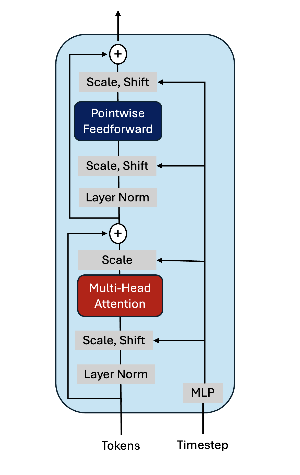
\includegraphics[width=\linewidth]{figures/layersync.png}
        \caption{Reference SiT stack used by fixed-pair internal alignment.}
    \end{subfigure}
    \hfill
    \begin{subfigure}[t]{0.55\linewidth}
        \centering
        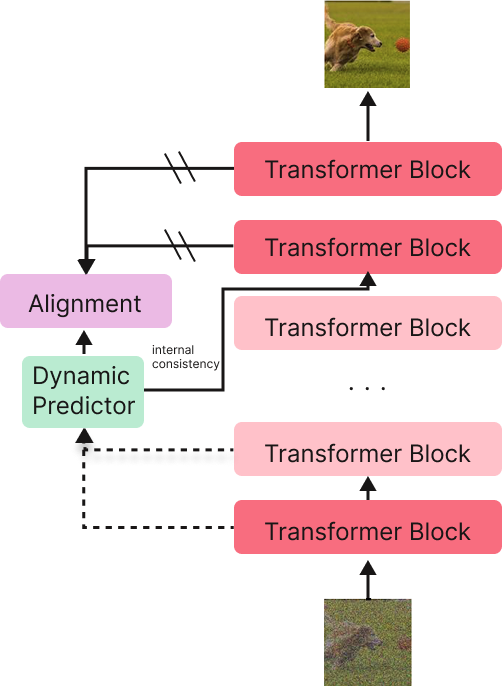
\includegraphics[height=0.34\textheight,keepaspectratio]{figures/resync.png}
        \caption{ReSync attaches a shared predictor to sampled source--target layers.}
    \end{subfigure}
    \caption{\textbf{SiT stack and ReSync attachment.} The backbone follows the same SiT block stack used by LayerSync~\citep{haghighi2026layersync}. ReSync keeps the stack unchanged and adds a training-time transition predictor between sampled depths.}
    \label{fig:appendix_sit_resync_architecture}
\end{figure}

\begin{table}[!htbp]
    \centering
    \caption{\textbf{SiT backbone details.} Placeholder table for backbone architecture details used in the main ImageNet experiments.}
    \label{tab:appendix_sit_architecture}
    \small
    \setlength{\tabcolsep}{5pt}
    \begin{tabular}{lccccc}
        \toprule
        Backbone & Layers & Hidden dim. & Heads & Patch size & Params \\
        \midrule
        \texttt{SiT-B/2} & \textbf{[TBD]} & \textbf{[TBD]} & \textbf{[TBD]} & 2 & 130M \\
        \texttt{SiT-L/2} & \textbf{[TBD]} & \textbf{[TBD]} & \textbf{[TBD]} & 2 & 458M \\
        \texttt{SiT-XL/2} & \textbf{[TBD]} & \textbf{[TBD]} & \textbf{[TBD]} & 2 & 675M \\
        \bottomrule
    \end{tabular}
\end{table}

\subsection{HumanML3D Setup}
\label{app:humanml3d_details}

HumanML3D contains text descriptions paired with 3D human-motion sequences~\citep{guo2022generating}. Following MDM~\citep{tevet2022mdm}, the baseline and ReSync runs use the same split, text encoder, motion representation, diffusion schedule, and evaluator. Because motion backbones are shallower than ImageNet SiT models, the selected transition pairs are reported explicitly.

\begin{table}[!htbp]
    \centering
    \caption{\textbf{HumanML3D setup.} Placeholder table for the exact motion-generation configuration.}
    \label{tab:appendix_humanml3d_setup}
    \small
    \setlength{\tabcolsep}{5pt}
    \begin{tabular}{lccccc}
        \toprule
        Method & Backbone layers & Iter. & Transition pairs & Evaluator & Metrics \\
        \midrule
        MDM & \textbf{[TBD]} & 600K & -- & \textbf{[TBD]} & FID, R-Precision \\
        MDM + ReSync & \textbf{[TBD]} & 600K & \textbf{[TBD]} & \textbf{[TBD]} & FID, R-Precision \\
        \bottomrule
    \end{tabular}
\end{table}

\subsection{Metric and Measurement Definitions}
\label{app:metric_definitions}

\subsubsection{Protocol Map for Main Tables and Figures}

We follow the common appendix convention of recent internal-alignment work: the main paper keeps tables and figures compact, while the appendix states the measurement protocol, sample count, normalization, and citations. \Cref{tab:appendix_main_protocol_map} maps each main result to the corresponding measurement rule.

\begin{table}[!htbp]
    \centering
    \caption{\textbf{Protocol map for main tables and figures.} Each main artifact reports a compact result; the appendix specifies how it is measured.}
    \label{tab:appendix_main_protocol_map}
    \scriptsize
    \setlength{\tabcolsep}{2.5pt}
    \renewcommand{\arraystretch}{0.9}
    \begin{tabular*}{0.98\linewidth}{@{\extracolsep{\fill}}p{0.22\linewidth}p{0.29\linewidth}p{0.31\linewidth}p{0.11\linewidth}@{}}
        \toprule
        Main artifact & Quantity & Protocol & Citation \\
        \midrule
        \Cref{tab:imagenet_no_cfg,tab:imagenet_cfg} & FID, IS, precision, recall & Generate the stated number of samples with matched sampler, VAE, reference statistics, and CFG setting; use the same evaluator for all rows. & \citep{heusel2017gans,salimans2016improved,kynkaanniemi2019precision} \\
        \Cref{tab:humanml3d_results} & FID, R-Precision & Use the standard HumanML3D evaluator, split, text encoder, and motion representation for baseline and ReSync. & \citep{guo2022generating,tevet2022mdm} \\
        \Cref{tab:resync_ablation} & FID-10K & Use the same TPU budget, batch size, iterations, sampler, VAE, and reference statistics; only objective terms change. & \citep{heusel2017gans} \\
        \Cref{fig:cosine_squared_heatmap} & Layer cosine heatmap & Flatten activations over images and spatial tokens, normalize token features, average cosine similarity over sampled data and timesteps. & \citep{kornblith2019similarity,raghu2021visiontransformers} \\
        \Cref{tab:pair_sampling_ablation} & Grouped prediction error & Train with uniform layer-pair sampling, then group $\mathcal{L}_{\mathrm{pred}}$ by layer gap, source layer, or timestep range. & this work \\
        \Cref{fig:representation_analysis} & Linear probes, segmentation probe, DINOv2 CKA & Freeze backbone features, train lightweight probes per layer, and compute CKA to DINOv2 features on matched images and timesteps. & \citep{deng2009imagenet,everingham2010pascal,oquab2023dinov2,kornblith2019similarity} \\
        \bottomrule
    \end{tabular*}
\end{table}

Standard generation metrics follow the cited benchmark protocols. FID compares Gaussian approximations of real and generated Inception features,
\begin{equation}
\operatorname{FID}
=
\|\mu_r-\mu_g\|_2^2
+
\operatorname{Tr}\left(
\Sigma_r+\Sigma_g
-2(\Sigma_r\Sigma_g)^{1/2}
\right),
\end{equation}
where lower is better. IS is computed using the Inception classifier convention of \citet{salimans2016improved}. Precision and recall follow the improved generative-model support estimate of \citet{kynkaanniemi2019precision}. For HumanML3D, FID uses motion-evaluator embeddings and R-Precision reports whether the matching text appears in the top retrieved candidates under the standard HumanML3D/MDM evaluation protocol~\citep{guo2022generating,tevet2022mdm}.

For hidden-state diagnostics, let $X,Y\in\mathbb{R}^{M\times C}$ denote flattened token activations, where $M$ indexes images and spatial tokens. Activation RMS is $\sqrt{(MC)^{-1}\sum_{m,c}X_{m,c}^2}$, and token norm is $M^{-1}\sum_m\|X_{m,:}\|_2$. Pairwise cosine heatmaps use row-normalized features $\tilde X_m=X_m/(\|X_m\|_2+\varepsilon)$ and report the average token cosine between layer pairs. Linear CKA is
\begin{equation}
\operatorname{CKA}(X,Y)
=
\frac{\|X_c^{\top}Y_c\|_F^2}
{\|X_c^{\top}X_c\|_F\|Y_c^{\top}Y_c\|_F+\varepsilon},
\end{equation}
following \citet{kornblith2019similarity}; we use it for transformer-layer comparisons in the same diagnostic spirit as \citet{raghu2021visiontransformers}. Stable rank is $\|Z\|_F^2/\|Z\|_2^2$ after channelwise normalization, and PCA visualizations use the leading principal components of the same normalized activations. Pseudo-mask IoU and Boundary-F1 compare spatial structures recovered from activations with a reference partition or boundary map. Transition prediction error is
\begin{equation}
E_{\mathrm{pred}}(a,b)
=
\mathbb{E}_{x,t}
\left[
d\left(g_\psi(A_a^t;a,b,t),\operatorname{sg}(A_b^t)\right)
\right],
\end{equation}
where $d$ is tokenwise cosine distance unless stated otherwise. The grouped prediction-error tables in \Cref{tab:pair_sampling_ablation} average this quantity over the specified layer-gap bin, source-layer bin, or timestep bin. Linear classification probes use frozen intermediate features and a linear head; segmentation probes use frozen spatial features and a linear pixel classifier on PASCAL VOC~\citep{everingham2010pascal}. For diagnostics not tied to a named benchmark, captions report the normalization axes, sample count, timestep range, layer-pair rule, and whether higher or lower is better.

\section{Additional Ablations and Scaling}
\label{app:resync_ablation_protocols}

The main ablation tables isolate the components needed for ReSync. This appendix reports the broader sweeps that are useful for interpretation but too detailed for the main paper.

\subsection{Appendix-Only Control Map}

The following controls support the main ablation story without becoming separate claims. They document configuration choices, sensitivity to schedules and weights, and supplementary visual diagnostics.

\begin{table}[!htbp]
    \centering
    \caption{\textbf{Appendix-only controls.} Placeholder map for secondary experiments kept outside the main ablation section.}
    \label{tab:appendix_control_map}
    \scriptsize
    \setlength{\tabcolsep}{3pt}
    \renewcommand{\arraystretch}{0.9}
    \begin{tabular*}{0.98\linewidth}{@{\extracolsep{\fill}}p{0.24\linewidth}p{0.36\linewidth}p{0.28\linewidth}@{}}
        \toprule
        Control & Purpose & Report \\
        \midrule
        Standard vs. transition-interface inference & Check the optional inference interface separately from the standard-sampling main claim & FID-4K / FID-10K, cost \\
        Timestep PCA & Visualize how representations and predictor outputs evolve across denoising time & PCA maps, timestep panels \\
        Predictor output vs. target layer & Check whether predicted states recover target-layer structure & PCA, cosine heatmap, CKA \\
        Architecture and strategy config & Document the final predictor architecture and pair-selection rule & ConvNeXt-style predictor / selected schedule \\
        Lambda tuning & Set the ReSync weight without changing the main recipe & FID, prediction error, stability \\
        Max-gap and pair schedule & Separate max layer gap from timestep schedule effects & FID, $\mathcal{L}_{\mathrm{pred}}$ \\
        Qualitative samples & Show matched-seed visual differences & Image grids \\
        \bottomrule
    \end{tabular*}
\end{table}

\subsection{Transition-Pair Selection}

We sweep source and target blocks while keeping compute, batch size, and training iterations fixed. Generation metrics are reported together with transition-level metrics, since a low prediction loss can also indicate that the pair is easy.

\begin{table}[!htbp]
    \centering
    \caption{\textbf{Ablation on transition-pair selection.} Placeholder for testing source/target ranges and layer gaps.}
    \label{tab:appendix_pair_selection}
    \small
    \setlength{\tabcolsep}{4pt}
    \begin{tabular}{lccccc}
        \toprule
        Backbone & Source range & Target range & Gap & FID $\downarrow$ & Comp. error $\downarrow$ \\
        \midrule
        \textbf{[TBD]} & weak blocks & middle blocks & short & \textbf{[TBD]} & \textbf{[TBD]} \\
        \textbf{[TBD]} & weak blocks & middle blocks & medium & \textbf{[TBD]} & \textbf{[TBD]} \\
        \textbf{[TBD]} & weak blocks & decoder blocks & long & \textbf{[TBD]} & \textbf{[TBD]} \\
        \textbf{[TBD]} & random valid pairs & mixed & mixed & \textbf{[TBD]} & \textbf{[TBD]} \\
        \bottomrule
    \end{tabular}
\end{table}

\subsection{Timestep Coverage and Conditioning}

This ablation separates which timesteps receive the transition loss from whether the predictor is explicitly conditioned on $t$.

\begin{table}[!htbp]
    \centering
    \caption{\textbf{Ablation on timestep coverage and conditioning.} Placeholder for testing transition prediction across denoising time.}
    \label{tab:appendix_timestep_ablation}
    \small
    \setlength{\tabcolsep}{4pt}
    \begin{tabular}{lcccc}
        \toprule
        Timestep coverage & Time cond. & FID $\downarrow$ & Prediction error $\downarrow$ & Comp. error $\downarrow$ \\
        \midrule
        25\% & \checkmark & \textbf{[TBD]} & \textbf{[TBD]} & \textbf{[TBD]} \\
        50\% & \checkmark & \textbf{[TBD]} & \textbf{[TBD]} & \textbf{[TBD]} \\
        100\% & -- & \textbf{[TBD]} & \textbf{[TBD]} & \textbf{[TBD]} \\
        100\% & \checkmark & \textbf{[TBD]} & \textbf{[TBD]} & \textbf{[TBD]} \\
        \bottomrule
    \end{tabular}
\end{table}

\subsection{Predictor Capacity and Optimization Controls}

We compare small and large predictors, pair-specific projectors, and matched-learning-rate controls. These runs separate cross-depth transition learning from raw auxiliary capacity.

\begin{table}[!htbp]
    \centering
    \caption{\textbf{Predictor capacity and optimization controls.} Placeholder for separating transition learning from capacity or optimization effects.}
    \label{tab:appendix_predictor_capacity_controls}
    \scriptsize
    \setlength{\tabcolsep}{3pt}
    \begin{tabular}{lccccc}
        \toprule
        Variant & Pred. params & Aux. weight & FID $\downarrow$ & Align. $\downarrow$ & Comp. $\downarrow$ \\
        \midrule
        Baseline & -- & -- & \textbf{[TBD]} & -- & -- \\
        Small shared predictor & \textbf{[TBD]} & \textbf{[TBD]} & \textbf{[TBD]} & \textbf{[TBD]} & \textbf{[TBD]} \\
        Large shared predictor & \textbf{[TBD]} & \textbf{[TBD]} & \textbf{[TBD]} & \textbf{[TBD]} & \textbf{[TBD]} \\
        Pair-specific projectors & \textbf{[TBD]} & \textbf{[TBD]} & \textbf{[TBD]} & \textbf{[TBD]} & \textbf{[TBD]} \\
        Matched learning-rate baseline & -- & \textbf{[TBD]} & \textbf{[TBD]} & -- & -- \\
        \bottomrule
    \end{tabular}
\end{table}

\subsection{Lambda, Max-Gap, and Schedule Controls}

These controls tune the final recipe without changing the main ReSync mechanism. We report them in the appendix because they select practical hyperparameters and keep the main paper focused.

\begin{table}[!htbp]
    \centering
    \caption{\textbf{Lambda and schedule controls.} Placeholder for tuning the ReSync weight, maximum layer gap, and pair/timestep schedule.}
    \label{tab:appendix_lambda_schedule_controls}
    \scriptsize
    \setlength{\tabcolsep}{3pt}
    \renewcommand{\arraystretch}{0.9}
    \begin{tabular*}{0.96\linewidth}{@{\extracolsep{\fill}}lcccc@{}}
        \toprule
        Setting & $\lambda_{\mathrm{sync}}$ & Max gap & Pair / timestep schedule & FID $\downarrow$ \\
        \midrule
        Low weight & \textbf{[TBD]} & \textbf{[TBD]} & final & \textbf{[TBD]} \\
        Default & \textbf{[TBD]} & \textbf{[TBD]} & final & \textbf{[TBD]} \\
        High weight & \textbf{[TBD]} & \textbf{[TBD]} & final & \textbf{[TBD]} \\
        Short max gap & default & \textbf{[TBD]} & final & \textbf{[TBD]} \\
        Long max gap & default & \textbf{[TBD]} & final & \textbf{[TBD]} \\
        Alternative schedule & default & default & \textbf{[TBD]} & \textbf{[TBD]} \\
        \bottomrule
    \end{tabular*}
\end{table}

\subsection{Scaling Across Backbones and Model Sizes}
\label{app:scaling_experiments}

Scaling runs test whether the same ReSync recipe transfers across \texttt{B/2}, \texttt{L/2}, and \texttt{XL/2} backbones. The comparison uses matched training settings within each size.

\begin{figure}[!htbp]
    \centering
    \fbox{%
    \begin{minipage}[c][0.22\textheight][c]{0.88\linewidth}
        \centering
        \textbf{[PLACEHOLDER: training curves]}\\[0.5em]
        Plot baseline vs. ReSync across training iterations. Suggested axes: FID, validation loss, or representation metric.
    \end{minipage}}
    \caption{\textbf{Training dynamics across model scales.} Placeholder for convergence curves comparing baseline and ReSync-augmented backbones.}
    \label{fig:appendix_training_curves}
\end{figure}

\begin{table}[!htbp]
    \centering
    \caption{\textbf{ReSync across model sizes.} Placeholder table for comparing baseline and ReSync variants under matched training settings.}
    \label{tab:appendix_model_scaling}
    \begin{tabular}{lcccc}
        \toprule
        Backbone & Params & Objective & FID $\downarrow$ & Throughput / steps \\
        \midrule
        \texttt{B/2} & \textbf{[TBD]} & Baseline & \textbf{[TBD]} & \textbf{[TBD]} \\
        \texttt{B/2} & \textbf{[TBD]} & Baseline + ReSync & \textbf{[TBD]} & \textbf{[TBD]} \\
        \texttt{L/2} & \textbf{[TBD]} & Baseline & \textbf{[TBD]} & \textbf{[TBD]} \\
        \texttt{L/2} & \textbf{[TBD]} & Baseline + ReSync & \textbf{[TBD]} & \textbf{[TBD]} \\
        \texttt{XL/2} & \textbf{[TBD]} & Baseline & \textbf{[TBD]} & \textbf{[TBD]} \\
        \texttt{XL/2} & \textbf{[TBD]} & Baseline + ReSync & \textbf{[TBD]} & \textbf{[TBD]} \\
        \bottomrule
    \end{tabular}
\end{table}

\section{Representation and Transition Diagnostics}
\label{app:layer_statistics_projection}

This section collects the diagnostics behind \Cref{sec:representation_analysis} and the projection-as-transition probe in \Cref{tab:layersync_projector_probe}. The main paper reports the compact version; the appendix gives protocols, controls, and additional views.

\subsection{Diagnostic Protocol}
\label{app:diagnostic_protocol}

Diagnostics use the same checkpoints, dataset split, resolution, VAE, and layer sampling scheme as the main experiments. The comparison set is:
\begin{itemize}[leftmargin=*]
    \item baseline DiT/SiT backbone without auxiliary representation guidance;
    \item LayerSync-style direct cosine alignment;
    \item LayerSync-style alignment with a small projection head;
    \item pair-specific projectors for selected layer pairs;
    \item ReSync with a shared conditional transition predictor.
\end{itemize}
For each method, report layer pairs, timestep ranges, projection or predictor architecture, loss weights, and whether an EMA target is used. Source groups are defined by block index for a backbone with $L$ blocks: $\mathcal{S}_{\mathrm{early}}=\{1,\dots,\lfloor0.2L\rfloor\}$, $\mathcal{S}_{\mathrm{mid}}=\{\lfloor0.4L\rfloor,\dots,\lfloor0.6L\rfloor\}$, and $\mathcal{S}_{\mathrm{late}}=\{\lceil0.8L\rceil,\dots,L\}$.

\subsection{Layerwise Probe Protocol}

For the representation analysis in \Cref{sec:representation_analysis}, we report probes across all backbone blocks. Linear classification uses frozen hidden states with a lightweight linear head. Segmentation probes use the same frozen features with a linear pixel classifier after spatial reshaping. CKA compares centered token activations with DINOv2 features on the same images and timesteps. Matched-FID checkpoints are preferred for the main figure so that the layerwise comparison reflects representation organization under comparable sample quality.

\subsection{Predictor-Output Diagnostics}

These diagnostics compare the predicted target state with the actual target layer across layer depth and denoising time. They show whether the transition predictor recovers useful target-layer structure alongside the scalar prediction loss.

\begin{figure}[!htbp]
    \centering
    \fbox{%
    \begin{minipage}[c][0.24\textheight][c]{0.9\linewidth}
        \centering
        \textbf{[PLACEHOLDER: predictor-output diagnostics]}\\[0.5em]
        Panels: PCA of actual target layer, PCA of predictor output, timestep PCA,\\
        predictor-target cosine heatmap, and layerwise CKA.
    \end{minipage}}
    \caption{\textbf{Predictor output versus target layer.} Placeholder for visualizing whether the learned transition recovers target-layer structure across depth and denoising time.}
    \label{fig:appendix_predictor_output_diagnostics}
\end{figure}

\subsection{Layerwise Statistical Mismatch}
\label{app:layerwise_statistical_mismatch}

This diagnostic measures how representation statistics change across depth. We report RMS activation, token norm, channelwise variance, stable rank, effective rank, cosine similarity, SVCCA, and CKA by layer index and by layer distance. Larger shifts for distant pairs indicate stronger feature-space mismatch and make a learned transition interface more useful before the alignment signal reaches the backbone.

\begin{figure}[!htbp]
    \centering
    \fbox{%
    \begin{minipage}[c][0.22\textheight][c]{0.9\linewidth}
        \centering
        \textbf{[PLACEHOLDER: layerwise statistical mismatch]}\\[0.5em]
        Panels: RMS activation, variance, stable rank, cosine similarity, and CKA.\\
        Axes: layer index and layer distance; curves for baseline, LayerSync variants, and ReSync.
    \end{minipage}}
    \caption{\textbf{Layerwise statistical mismatch.} Placeholder for measuring how representation statistics change across depth and timestep.}
    \label{fig:appendix_layerwise_statistics}
\end{figure}

\subsection{Projection Capacity and Layer Gap}
\label{app:projection_capacity_layer_gap}

This ablation tests whether projection heads extract useful recoverable signal or simply absorb the auxiliary loss. The key comparison is direct alignment versus small and large projection heads across near and far layer pairs. A useful projection should improve generation and representation probes, along with local alignment loss.

\begin{figure}[!htbp]
    \centering
    \fbox{%
    \begin{minipage}[c][0.22\textheight][c]{0.9\linewidth}
        \centering
        \textbf{[PLACEHOLDER: projection capacity ablation]}\\[0.5em]
        Compare no projection, small projection, medium projection, and large projection.\\
        Report FID, alignment loss, representation probes, and training cost.
    \end{minipage}}
    \caption{\textbf{Projection capacity ablation.} Placeholder for testing whether projection capacity exposes useful signal across layer gaps.}
    \label{fig:appendix_projection_capacity}
\end{figure}

\begin{table}[!htbp]
    \centering
    \caption{\textbf{Near vs. far layer alignment.} Placeholder for evaluating whether projection heads and ReSync become more important as the layer gap increases.}
    \label{tab:appendix_near_far_alignment}
    \resizebox{\textwidth}{!}{%
    \begin{tabular}{lccccc}
        \toprule
        Method & Layer gap & Projection / transition & FID $\downarrow$ & Alignment loss $\downarrow$ & Consistency error $\downarrow$ \\
        \midrule
        Direct alignment & Near & -- & \textbf{[TBD]} & \textbf{[TBD]} & -- \\
        Direct alignment & Far & -- & \textbf{[TBD]} & \textbf{[TBD]} & -- \\
        Projection-augmented alignment & Near & Small projector & \textbf{[TBD]} & \textbf{[TBD]} & -- \\
        Projection-augmented alignment & Far & Small projector & \textbf{[TBD]} & \textbf{[TBD]} & -- \\
        Pair-specific projector & Far & Per-pair projector & \textbf{[TBD]} & \textbf{[TBD]} & \textbf{[TBD]} \\
        ReSync & Near & Shared transition & \textbf{[TBD]} & \textbf{[TBD]} & \textbf{[TBD]} \\
        ReSync & Far & Shared transition & \textbf{[TBD]} & \textbf{[TBD]} & \textbf{[TBD]} \\
        \bottomrule
    \end{tabular}}
\end{table}

\subsection{Layout-Recoverable Spatial Information}
\label{app:layout_recoverable_information}

Spatial probes ask whether activations preserve layout in a recoverable form. We convert activations into spatial partitions or boundaries and compare them with DINO-derived pseudo masks, image edges, or object masks when available. Same-image, different-image, and token-shuffle controls check whether the score reflects image-specific layout.

\begin{figure}[!htbp]
    \centering
    \fbox{%
    \begin{minipage}[c][0.24\textheight][c]{0.9\linewidth}
        \centering
        \textbf{[PLACEHOLDER: layout-recoverable spatial information]}\\[0.5em]
        Panels: PCA maps, spatial-normalized PCA maps, DINO pseudo-mask IoU, Boundary-F1,\\
        region agreement, and same/different-image controls.
    \end{minipage}}
    \caption{\textbf{Layout-recoverable spatial information.} Placeholder for measuring spatial structure in internal activations alongside raw feature similarity.}
    \label{fig:appendix_layout_recoverable}
\end{figure}

\subsection{Transition Generalization}
\label{app:transition_generalization}

This diagnostic distinguishes a shared transition interface from a collection of pair-specific heads. We train on a subset of layer pairs and evaluate prediction and composition error on held-out pairs at the same denoising timestep. Lower held-out and composition errors indicate that the shared predictor captures reusable cross-depth structure.

\begin{table}[!htbp]
    \centering
    \caption{\textbf{Held-out transition generalization.} Placeholder for testing whether ReSync generalizes across unseen layer pairs better than pair-specific projectors.}
    \label{tab:appendix_transition_generalization}
    \resizebox{\textwidth}{!}{%
    \begin{tabular}{lccc}
        \toprule
        Method & Held-out layer error $\downarrow$ & Composition error $\downarrow$ & FID $\downarrow$ \\
        \midrule
        Pair-specific projector & \textbf{[TBD]} & \textbf{[TBD]} & \textbf{[TBD]} \\
        Shared transition without consistency & \textbf{[TBD]} & \textbf{[TBD]} & \textbf{[TBD]} \\
        ReSync shared transition & \textbf{[TBD]} & \textbf{[TBD]} & \textbf{[TBD]} \\
        \bottomrule
    \end{tabular}}
\end{table}

\section{Qualitative Examples}
\label{app:qualitative_examples}

Qualitative examples use matched noise, sampler, guidance, and checkpoints across baseline, Dispersive, LayerSync-style alignment, and ReSync. They supplement the quantitative metrics by showing visible failure modes and sample-level differences under the same random seed.

\begin{figure}[!htbp]
    \centering
    \fbox{%
    \begin{minipage}[c][0.24\textheight][c]{0.9\linewidth}
        \centering
        \textbf{[PLACEHOLDER: qualitative ImageNet samples]}\\[0.5em]
        Rows: baseline, Dispersive, LayerSync-style alignment, ReSync.\\
        Columns: matched class labels and identical initial noise.
    \end{minipage}}
    \caption{\textbf{Qualitative ImageNet comparison.} Placeholder for matched-seed samples used as supplementary visual evidence.}
    \label{fig:appendix_qualitative_samples}
\end{figure}


\newpage
\input{checklist}

\end{document}
